\chapter{Introduction}
\label{chp:introduction}

\section{Motivation}
The Internet-of-Things (IoT) is a promising vision which enables billions or trillions of sensor devices to be connected \cite{flicker}. A common bottleneck for such devices is the energy supply. Batteries are large, expensive, heavy and wear out after several years.  %todo add references + note that replacement is an issue

A sustainable solution is energy harvesting where a device collects it's energy from the environment for instance solar, radio frequency (RF), thermal or kinetic energy.

However, developing software for such devices comes with a challenge. Environmental energy can be scarce, causing frequent power failures \cite{tpcthesis}. This contrasts with the standard assumption that programs run continuously throughout execution. The programmer has to take care of this intermittent behavior by for instance storing data to non-volatile memory at certain intervals. The available energy tends to be random, making it difficult to predict how long a program can execute before the next power failure. 

It is hard to conduct repeatable tests due to the random nature of the energy source. While comparing two algorithms, it is impossible to conclude that one algorithm outperforms the other without knowing how much the difference in available energy contributed to the result.

\section{Research goal and contributions}

\textit{Provide a remote accessible testbed to accelerate the development in applications for batteryless devices for those who do not have the resources or tools them selfs and assist developers in finding bugs caused by intermittent behavior.}\\

The proposed architecture of the testbed is shown in Figure \ref{fig:architecture}

Flicker \cite{flicker} would be an ideal platform to use as device under test (DUT), because it supports many software configurable peripherals and has the MSP430 as its core, a common micro controller in low-power applications. An WISP \cite{wisp} could be a possible DUT.

Ekho \cite{ekho} would complement this setup because it can emulate various energy harvesting conditions. An alternative to Ekho would be toggling the power source by a configurable frequency and duty-cycle. Besides emulating, real energy harvesting sources can be used. A configurable light source can be used to power solar panels. An RFID reader can be used to harvest RF energy. 

Several methods can be used to track the progress and outcome of a test: serial console (printf), GPIO tracing (logic analyzer), memory dumping and a debugger (possibly energy aware \cite{edb}).

\begin{figure}[htb]
	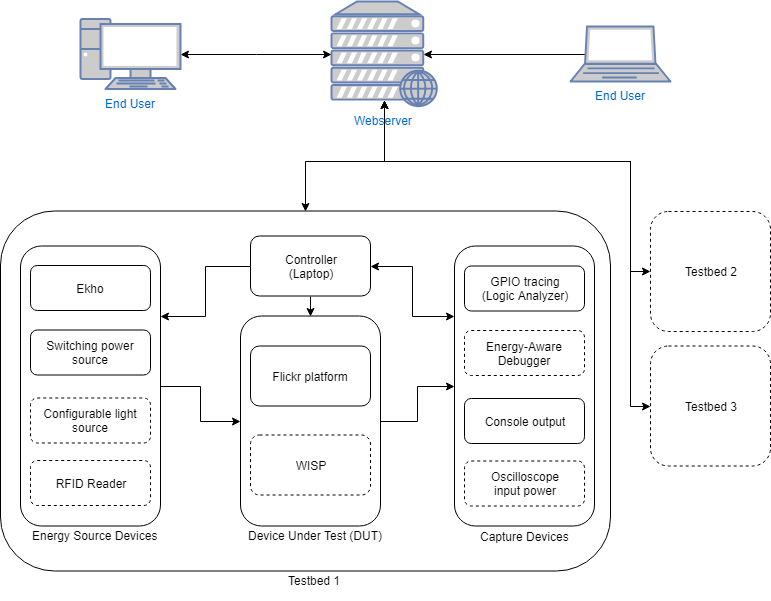
\includegraphics[width=\textwidth]{pics/TestbedArchitecture_v3}
	\caption{Proposed testbed architecture. The dotted lines show optional modules.}
	\label{fig:architecture}
\end{figure}

\section{Thesis outline}

\vspace{1\baselineskip}

\noindent
TODO ORGANISATIONAL DESCRIPTION OF THESIS

